\documentclass{article}

\usepackage{graphicx}
\usepackage{tikz}
\usepackage{tikzsymbols}
\usetikzlibrary{calc,patterns,shapes.geometric}
\pagestyle{empty}
\usepackage[margin=0pt]{geometry}
\geometry{papersize={14in,12in}}

\def\centerarc[#1](#2)(#3:#4:#5){\draw[#1] ($(#2)+({#5*cos(#3)},{#5*sin(#3)})$) arc (#3:#4:#5);}

\begin{document}
	\begin{figure}
		\centering
		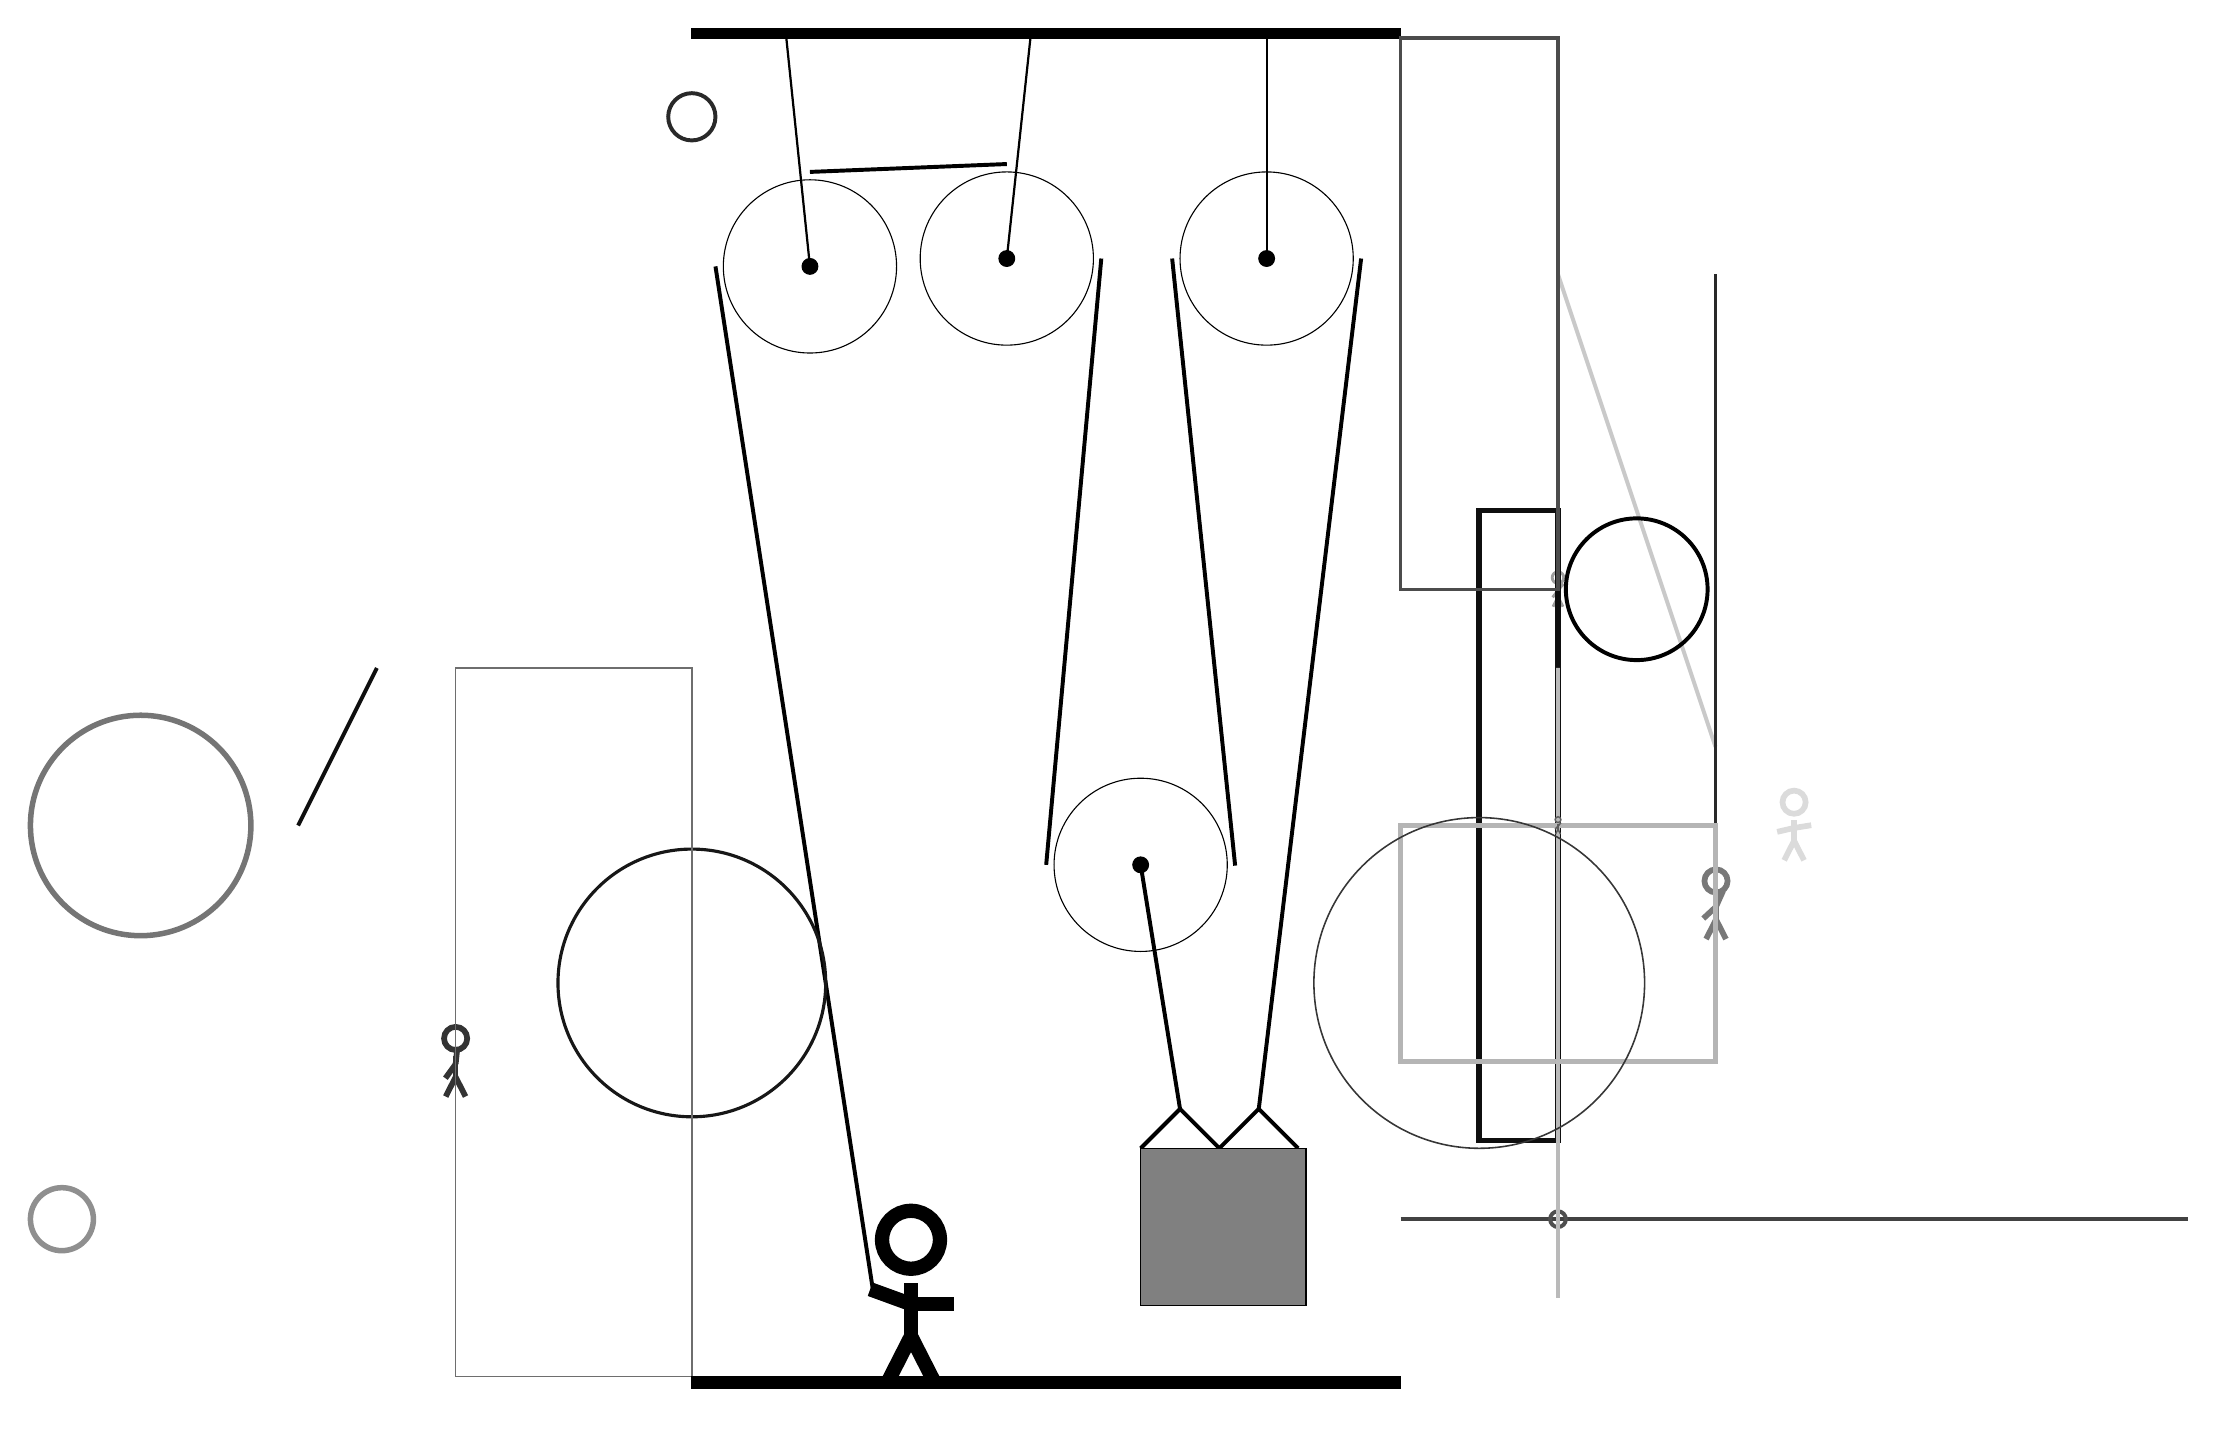
\begin{tikzpicture}
			%%%%% START %%%%%
			
			\draw[fill=black] (-3, 14) rectangle (6, 14.125);
			
			\draw (1, 11.2) circle (1.1);
			\draw[fill=black] (1, 11.2) circle (0.1);
			\draw[thick] (1, 11.2) -- (1.3, 14);
			
			\draw (4.3, 11.2) circle (1.1);
			\draw[fill=black] (4.3, 11.2) circle (0.1);
			\draw[thick] (4.3, 11.2) -- (4.3, 14);
			
			\draw (2.7, 3.5) circle (1.1);
			\draw[fill=black] (2.7, 3.5) circle (0.1);
			
			\draw[line width=0.5mm]  (2.7, -0.1) -- (3.2, 0.4) -- (3.7, -0.1) -- (4.2, 0.4) -- (4.7, -0.1);
			\draw[fill=black!50] (2.7, -0.1) rectangle (4.8, -2.1);
			
			\draw (-1.5, 11.1) circle (1.1);
			\draw[fill=black] (-1.5, 11.1) circle (0.1);
			\draw[thick] (-1.5, 11.1) -- (-1.8, 14);
			
			\draw[line width=0.5mm](-0.7, -1.9) --  (-2.7, 11.1);
			\centerarc[line width=0.5mm](-1.5, 11.1)(90:180:1.2000000000000002);
			\draw[line width=0.5mm](-1.5, 12.3) -- (1, 12.4);
			\centerarc[line width=0.5mm](1, 11.2)(0:90:1.2000000000000002);
			\draw[line width=0.5mm](2.2, 11.2) -- (1.5, 3.5);
			\centerarc[line width=0.5mm](2.7, 3.5)(180:370:1.2000000000000002);
			\draw[line width=0.5mm] (3.9, 3.49) -- (3.1, 11.2);
			\centerarc[line width=0.5mm](4.3, 11.2)(0:180:1.2000000000000002);
			\draw[line width=0.5mm](4.2, 0.4) -- (5.5, 11.2);
			\draw[line width=0.5mm] (3.2, 0.4) -- (2.7, 3.5);
			
			\node at (-0.2, -2) {\Strichmaxerl[10][-20][0]};
			
			\draw[line width=0.5mm, color=black!21](8, 11) -- (10, 5);
			
			\draw [line width=0.4mm, color=black!91](-3, 2) circle (1.7);
			\draw[line width=0.5mm, color=black!84](10, 4) -- (10, 11);
			\draw[line width=0.5mm, color=black!74](6, -1) -- (16, -1);
			\draw[line width=0.5mm, color=black!94](-8, 4) -- (-7, 6);
			\draw [line width=0.5mm, color=black!69](8, -1) circle (0.1);
			
			\node[line width=0.5mm, color=black!38] at (8, 7) {\Strichmaxerl[2][52][51]};
			
			\draw[line width=0.7mm, color=black!94] (8, 8) rectangle (7, 0);
			\node[line width=0.5mm, color=black!53] at (10, 3) {\Strichmaxerl[4][43][66]};
			\draw [line width=0.5mm, color=black!100](9, 7) circle (0.9);
			
			\draw[line width=0.4mm, color=black!70] (8, 14) rectangle (6, 7);
			\draw [line width=0.7mm, color=black!54](-10, 4) circle (1.4);
			\node[line width=0.3mm, color=black!14] at (11, 4) {\Strichmaxerl[4][13][9]};
			
			\draw [line width=0.5mm, color=black!84](-3, 13) circle (0.3);
			\draw[line width=0.6mm, color=black!29] (6, 4) rectangle (10, 1);
			\node[line width=0.5mm, color=black!80] at (-6, 1) {\Strichmaxerl[4][54][84]};
			
			\draw[line width=0.4mm, color=black!27] (8, 6) rectangle (8, -2);
			
			\draw [line width=0.2mm, color=black!79](7, 2) circle (2.1);
			\draw [line width=0.7mm, color=black!44](-11, -1) circle (0.4);
			\draw[line width=0.2mm, color=black!57] (-3, 6) rectangle (-6, -3);
			\node[line width=0.4mm, color=black!64] at (8, 4) {\Strichmaxerl[1][46][48]};
			
			
			\draw[fill=black] (-3, -3) rectangle (6, -3.15);
			
			%%%%% END %%%%%
		\end{tikzpicture}
	\end{figure}	
\end{document}